\problemname{Chocolates}

\textit{``My mom always said life was like a box of chocolates. You never know what you're gonna get."}\\

Forrest Gump is a young boy who goes to Greenbow County Central School. As a child, he enjoys running, dancing by swinging his hips, and eating chocolates. Most of all, he enjoys spending time with his best friend Jenny. However, Forrest isn't the brightest boy by conventional means. While he fully embraces the life wisdom that his mama often imparts (such as through analogies with boxes of chocolates), he still has trouble keeping up with his classes.\\

Forrest's math class is currently learning about shapes, specifically polygons. Forrest is falling behind because he doesn't really understand what a polygon is. Jenny knows that if Forrest doesn't keep up, his mama would have to take drastic measures to prevent the crooked principal, Mr. Hancock, from transferring Forrest to a special school. As such, Jenny has decided take Forrest's schooling into her own hands.\\

Jenny has decided to use something that Forrest understands to explain polygons to him. She picks up a box of square chocolates and empties the pieces onto a napkin, leaving an empty box with $R$ rows and $C$ columns of empty cells. She places a single piece of chocolate in the box and says ``\textit{With one chocolate here, I've made a square. A square is a polygon, Forrest.}"

\begin{center}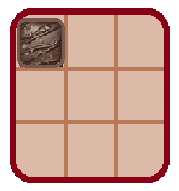
\includegraphics[width=100pt]{chocolates1.png}\end{center}

Jenny added two more chocolates around the first one and said, ``\textit{We still have here a polygon, because we can trace a border around the chocolates without our fingers leaving the surface of the box.}"

\begin{center}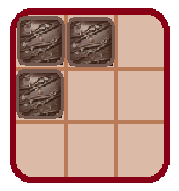
\includegraphics[width=100pt]{chocolates2.png}\end{center}

Jenny adds some more chocolates, filling up the entire box except a hole in the middle. ``\textit{Now Forrest, no matter how we trace the outside box, there will always be a hole we can never draw unless our finger leaves the surface. So this here ain't a polygon.}"

\begin{center}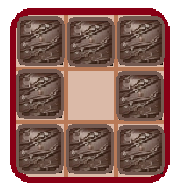
\includegraphics[width=100pt]{chocolates3.png}\end{center}

Jenny removes a chocolate from the corner and says, ``\textit{Now we're back to a polygon again! As long as we can trace the border of our chocolates without crossing over where we already traced, we have ourselves here a polygon. As we trace, we can even have two corners barely touch, so long as we don't overlap any border line we've already gone over.}".

\begin{center}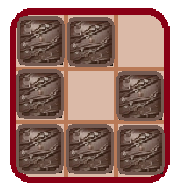
\includegraphics[width=100pt]{chocolates4.png}\end{center}

``\textit{That's amazing Jenny. Even with just a small box like that, it seems like you can make so many of 'em}", said Forrest.\\

``\textit{That's right Forrest!}", said Jenny. ``\textit{There's so many ways to make a polygon using this box of chocolates, if I just made one at random and had you guess, you truly are never gonna know what you're gonna get!}"\\

``\textit{Well, Jenny. Just how many ways do you think are there?}" asked Forrest.\\

``\textit{Hmm, I'm not quite sure about that Forrest.}" Jenny thought for a moment. "\textit{You really have me stumped.}"\\

Jenny wants to impress Forrest with the answer. Given the dimensions of the chocolate box, can you help her count the number of ways? For example, a 2 by 2 chocolate box has 13 ways of forming a polygon:
\begin{verbatim}
   x.   .x   ..   ..   xx   x.   ..   .x   xx   .x   xx   x.   xx
   ..   ..   x.   .x   ..   x.   xx   .x   x.   xx   .x   xx   xx
\end{verbatim}

\section*{Input}
The first and only line of input consists of two space-separated integers $R$ and $C$ ($1 \leq R, C \leq 4$), specifying the dimensions of the box of chocolates.

\section*{Output}
Print, on a single line, the number of different ways that chocolates can form a single polygon in the box. Note that if the same polygon can be placed at multiple different places in the box, then all of those ways are counted separately towards the answer.\\
